\documentclass[letterpaper,10pt]{article}

\usepackage{enumitem}
\usepackage{titling}
\usepackage{listings,listings-rust}
\usepackage{url}
\usepackage{soul}
\usepackage{hyperref}
\usepackage{setspace}
\usepackage{subfig}
\usepackage{sectsty}
\usepackage{pdfpages}
\usepackage{colortbl}
\usepackage{multirow}
\usepackage{multicol}
\usepackage{relsize}
\usepackage{amsmath}
\usepackage{wasysym}
\usepackage{fancyvrb}
\usepackage[yyyymmdd]{datetime}
\usepackage{amsmath,amssymb,amsthm,graphicx,xspace}
\usepackage[titlenotnumbered,noend,noline]{algorithm2e}
\usepackage[compact]{titlesec}
\usepackage{XCharter}
\usepackage[T1]{fontenc}
\usepackage[scaled]{beramono}
\usepackage[normalem]{ulem}
\usepackage{booktabs}
\usepackage{tikz}
\usetikzlibrary{arrows.meta,automata,shapes,trees,matrix,chains,scopes,positioning,calc,decorations.pathreplacing}
\tikzstyle{block} = [rectangle, draw, fill=blue!20, 
    text width=2.5em, text centered, rounded corners, minimum height=2em]
\tikzstyle{bw} = [rectangle, draw, fill=blue!20, 
    text width=4em, text centered, rounded corners, minimum height=2em]

\definecolor{namerow}{cmyk}{.40,.40,.40,.40}
\definecolor{namecol}{cmyk}{.40,.40,.40,.40}
\renewcommand{\dateseparator}{-}

\let\LaTeXtitle\title
\renewcommand{\title}[1]{\LaTeXtitle{\textsf{#1}}}

\lstset{basicstyle=\footnotesize\ttfamily,breaklines=true}

\newcommand{\CPP}{C\nolinebreak\hspace{-.05em}\raisebox{.4ex}{\tiny\bf +}\nolinebreak\hspace{-.10em}\raisebox{.4ex}{\tiny\bf +}}
\def\CPP{{C\nolinebreak[4]\hspace{-.05em}\raisebox{.4ex}{\tiny\bf ++}}}

\newcommand{\handout}[5]{
  \noindent
  \begin{center}
  \framebox{
    \vbox{
      \hbox to 5.78in { {\bf ECE459: Programming for Performance } \hfill #2 }
      \vspace{4mm}
      \hbox to 5.78in { {\Large \hfill #4  \hfill} }
      \vspace{2mm}
      \hbox to 5.78in { {\em #3 \hfill \today} }
    }
  }
  \end{center}
  \vspace*{4mm}
}

\newcommand{\lecture}[3]{\handout{#1}{#2}{#3}{Lecture#1}}
\newcommand{\tuple}[1]{\ensuremath{\left\langle #1 \right\rangle}\xspace}

\addtolength{\oddsidemargin}{-1.000in}
\addtolength{\evensidemargin}{-0.500in}
\addtolength{\textwidth}{2.0in}
\addtolength{\topmargin}{-1.000in}
\addtolength{\textheight}{1.75in}
\addtolength{\parskip}{\baselineskip}
\setlength{\parindent}{0in}
\renewcommand{\baselinestretch}{1.5}
\newcommand{\term}{Winter 2020}

\singlespace


\begin{document}

\lecture{15 --- Cache Coherency}{\term}{Patrick Lam \& Jeff Zarnett}

\section*{Cache Coherency}

\begin{center}
    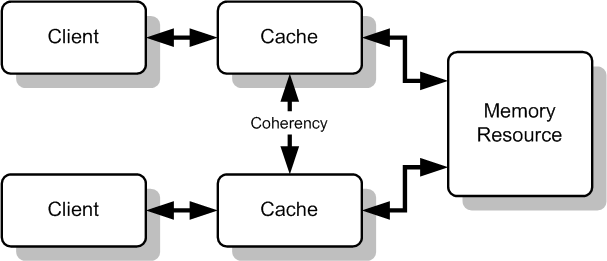
\includegraphics[width=0.5\textwidth]{images/coherency}

\hfill ---Wikipedia
\end{center}

We talked about memory ordering and fences last time.  Today we'll
look at what support the architecture provides for memory ordering, in
particular in the form of cache coherence. Since this isn't an
architecture course, we'll look at this material more from the point
of view of a user, not an implementer.

The problem is of course that each CPU might have its own cache and if it does then these data may be out of sync. The simplest method, and a horrible solution, is to declare some read/write variables as being non-cacheable (is that a word? Uncacheable?...). The compiler and OS and such will require the data to be read from memory always. Think of this as being like \texttt{volatile} (which prevented a variable from being put in a register), just moved up a level to preventing the variable from being put in a cache. This will obviously result in lower cache hit ratios, increased bus traffic, and terrible, terrible performance. Let's avoid that. What we want instead is coherency.

Cache coherency means that:
  \begin{itemize}
    \item the values in all caches are consistent; and
    \item to some extent, the system behaves as if all CPUs are using shared memory.
  \end{itemize}
  

\paragraph{Cache Coherence Example.} We will use this example to illustrate
different cache coherence algorithms and how they handle the same situation.

Initially in main memory: {\tt x = 7}.

  \begin{enumerate}
    \item {\tt CPU1} reads x, puts the value in its cache.
    \item {\tt CPU3} reads x, puts the value in its cache.
    \item {\tt CPU3} modifies {\tt x := 42}
    \item {\tt CPU1} reads x \ldots ~from its cache?
    \item {\tt CPU2} reads x. Which value does it get?
  \end{enumerate}

Unless we do something, {\tt CPU1} is going to read invalid data.

\paragraph{High-Level Explanation of Snoopy Caches.} The simplest way to ``do something''
is to use Snoopy caches~\cite{snoopycache}. No, not this kind of Snoopy (sadly):

\begin{center}
	
\includegraphics[width=0.25\textwidth]{images/peanuts-snoopy1.jpg}
\end{center}

This is a distributed approach; no centralized state is maintained. Each cache with a copy of data from a block of physical memory knows whether it is shared or not. All the CPUs are connected to a shared bus, and each CPU has its own cache controller. Whenever a CPU issues a memory write, the other CPUs are watching (snooping around) to observe if that memory location is in their cache. If it is, then the CPU will need to take action.


\subsection*{Write-Through Caches}
Let's put that into practice using write-through caches, the simplest type of
cache coherence.
  \begin{itemize}
    \item All cache writes are done to main memory.
    \item All cache writes also appear on the bus.
    \item If another CPU snoops and sees it has the same location in
      its cache, it will either {\it invalidate} or {\it update} the
      data.
  \end{itemize}
  
Invalidation is the most common protocol. It means the data in the cache of other CPUs is not updated, it's just noted as being out of date (invalid).  Normally, when you write to an invalidated location, you bypass the cache and go directly to memory (aka {\bf write no-allocate}). If we want to do a read and there's a miss, we can poke around in other caches to see who has the most recent cached version. This is a bit like going into a room and yelling ``Does anybody have block...?'', in some sort of multicast version of the card game ``Go Fish''. Regardless, the most recent value appears in memory, always.

There are also write broadcast protocols, in which case all versions in all caches get updated when there is a write to a shared block. But it uses lots of bandwidth and is not necessarily a good idea. It does, however prevent the costly cache miss that follows an invalidate. Sadly, as we are mere users and not hardware architects, we don't get to decide which is better; we just have to live with whichever one is on the hardware we get to use. Bummer.

\paragraph{Write-Through Protocol.}
The protocol for implementing such caches looks like this.
There are two possible states, {\bf valid} and {\bf invalid}, for each cached memory location.
Events are either from a processor ({\bf Pr}) or the {\bf Bus}. Actions will be either a \textbf{Rd} (read) or \textbf{Wr} (write).
We then implement the following state machine.

  \begin{center}
    \begin{tabular}{l|l|l|l}
      {\bf State} & {\bf Observed} & {\bf Generated} & {\bf Next State}\\ \hline
      Valid   & PrRd  &       & Valid\\
      Valid   & PrWr  & BusWr & Valid\\
      Valid   & BusWr &       & Invalid\\
      Invalid & PrWr  & BusWr & Valid\\
      Invalid & PrRd  & BusRd & Valid\\
    \end{tabular}
  \end{center}

\paragraph{Example.} For simplicity (this isn't an architecture course), assume all cache
      reads/writes are atomic. \footnote{If you're a hardware person, this line probably makes you cry. There's a whole lot that goes into making this work. There are potential write races, which have to be dealt with by contending for the bus and then completing the transaction, possibly restarting a command if necessary. If we have a split transaction bus it's really ugly, because we can have multiple interleaved misses. And down the rabbit hole we go.} Using the same example as before:

Initially in main memory: {\tt x = 7}.

  \begin{enumerate}
    \item {\tt CPU1} reads x, puts the value in its cache. {(valid)}
    \item {\tt CPU3} reads x, puts the value in its cache. {(valid)}
    \item {\tt CPU3} modifies {\tt x := 42}. {(write to memory)}
      \begin{itemize}
        \item {{\tt CPU1} snoops and marks data as invalid.}
      \end{itemize}
    \item {\tt CPU1} reads x, {from main memory. (valid)}
    \item {\tt CPU2} reads x, {from main memory. (valid)}
  \end{enumerate}

\subsection*{Write-Back Caches}
Let's try to improve performance. What if, in our example, {\tt CPU3} writes to {\tt x} 3 times? It's unpleasant to have to flush that to memory three times when we could do it only once. Let's try to delay the write to memory as long as possible. At minimum, we have to add a ``dirty'' bit, which indicates the our data has not yet been written to memory.

\paragraph{Write-Back Implementation.}
     The simplest type of write-back protocol (MSI) uses 3 states instead of 2:
      \begin{itemize}
        \item {\bf Modified}---only this cache has a valid copy; 
          main memory is {\bf out-of-date}.
        \item {\bf Shared}---location is unmodified, 
           up-to-date with main
          memory; 
          \quad may be present in other caches (also up-to-date).
        \item {\bf Invalid}---same as before.
      \end{itemize}
      
The initial state for a memory location, upon its first read, is ``shared''.
The implementation will only write the data to memory if another
processor requests it.
During write-back, a processor may read the data from the bus.

\paragraph{MSI Protocol.} Here, bus write-back (or flush) is {\bf BusWB}.
Exclusive read on the bus is {\bf BusRdX}.

\begin{center}
    \begin{tabular}{l|l|l|l}
      {\bf State} & {\bf Observed} & {\bf Generated} & {\bf Next State}\\ \hline
      Modified   & PrRd   &        & Modified\\
      Modified   & PrWr   &        & Modified\\
      Modified   & BusRd  & BusWB  & Shared\\
      Modified   & BusRdX & BusWB  & Invalid\\
      Shared     & PrRd   &        & Shared\\
      Shared     & BusRd  &        & Shared\\
      Shared     & BusRdX &        & Invalid\\
      Shared     & PrWr   & BusRdX & Modified\\
      Invalid    & PrRd   & BusRd  & Shared\\
      Invalid    & PrWr   & BusRdX & Modified\\
    \end{tabular}
\end{center}

\paragraph{MSI Example.} Using the same example as before:

Initially in main memory: {\tt x = 7}.

  \begin{enumerate}
    \item {\tt CPU1} reads x from memory. {(BusRd, shared)}
    \item {\tt CPU3} reads x from memory. {(BusRd, shared)}
    \item {\tt CPU3} modifies {\tt x = 42}:
      \begin{itemize}
        \item {Generates a BusRdX.}
        \item {{\tt CPU1} snoops and invalidates x.}
      \end{itemize}
    \item {\tt CPU1} reads x:
      \begin{itemize}
        \item {Generates a BusRd.}
        \item {{\tt CPU3} writes back the data and sets x to shared.}
        \item {{\tt CPU1} reads the new value from the bus as shared.}
      \end{itemize}
    \item {\tt CPU2} reads x from memory. {(BusRd, shared)}
  \end{enumerate}

\subsection*{An Extension to MSI: MESI}
    The most common protocol for cache coherence is MESI.
    This protocol adds yet another state:
      \begin{itemize}
        \item {\bf Modified}---only this cache has a valid copy; 
 main memory is {\bf out-of-date}.
        \item {\bf Exclusive}---only this cache has a valid copy; 
 main memory is {\bf up-to-date}.
        \item {\bf Shared}---same as before.
        \item {\bf Invalid}---same as before.
      \end{itemize}

    MESI allows a processor to modify data exclusive to it, without
    having to communicate with the bus.  MESI is safe. The key is that
    if memory is in the E state, no other processor has the data.

\subsection*{MSEIF: Even More States!}

    MESIF (used in latest i7 processors):
      \begin{itemize}
        \item {\bf Forward}---basically a shared state; but, current
          cache is the only one that will respond to a request to
          transfer the data.
      \end{itemize}

    Hence: a processor requesting data that is already shared or exclusive will
      only get one response transferring the data. This permits more efficient usage of the bus.

\subsection*{Cache coherence vs flush}

\begin{quote}
Cache coherency seems to make sure my data is consistent. Why do I have
to have something like flush or fence?
\end{quote}

Sadly, no. Cache coherence isn't enough. Writes may be to registers rather than
memory, and those won't be coherent. Use fences or flushes.

\begin{quote}
Well, I read that {\tt volatile} variables aren't stored in registers,
    so then am I okay?
\end{quote}

Again, sadly, no. Recall that {\tt volatile} in C was only designed to~\cite{pr:volatile}:
      \begin{itemize}
        \item Allow access to memory mapped devices.
        \item Allow uses of variables between {\tt setjmp} and {\tt longjmp}.
        \item Allow uses of {\tt sig\_atomic\_t} variables in signal handlers.
      \end{itemize}

All of these things apply to single-threaded situations or cases where the compiler has re-ordered some steps. Remember, things can also be reordered by the compiler, and {\tt
  volatile} doesn't prevent reordering. Also, it's likely your
variables could be in registers the majority of the time, except in
critical areas. All that volatile does is tell the compiler that an access of that variable should go to memory, not a register.

\paragraph{Coherence summary.}
We saw four cache coherence protocols, from MSI through MESIF. There
are many other protocols for cache coherence, each with their own
trade-offs.

Recall: OpenMP flush acts as a {\bf memory barrier/fence} so the
      compiler and hardware don't reorder reads and writes. Neither cache coherence nor {\tt volatile} will save you. Barriers/fences/flushes might be expensive in terms of ``wasting time,'' but correctness is important.

\bibliographystyle{alphaurl}
\bibliography{459}


\end{document}
